\documentclass[manuscript]{aastex}
\usepackage{graphicx}	% For figures
\usepackage{natbib}	% For citet and citep
\usepackage{amsmath}	% for \iint
\usepackage{bbm}	% for blackboard bold numbers

\newcommand{\vdag}{(v)^\dagger}
\newcommand{\myemail}{bj.brewer@auckland.ac.nz}

\shorttitle{Probabilistic Stellar Catalogs}
\shortauthors{Brewer et al.}

\begin{document}

\title{Probabilistic Catalogs for Crowded Stellar Fields}

\author{Brendon J. Brewer}
\affil{Department of Statistics, The University of Auckland,
Private Bag 92019, Auckland 1142, New Zealand}

\author{David W. Hogg}
\affil{Center for Cosmology and Particle Physics, Department of Physics,
New York University, Washington Place, New York, NY, 10003, USA}

\and

\author{Daniel Foreman-Mackey}
\affil{Center for Cosmology and Particle Physics, Department of Physics,
New York University, Washington Place, New York, NY, 10003, USA}

\begin{abstract}We introduce a probabilistic (Bayesian) method for producing catalogs
from images of crowded stellar fields. The method is capable of handling the
challenges introduced by overlapping sources and is able to determine the luminosity
function of the stars even when the precise luminosity of each star is uncertain.
This is in contrast with standard techniques which make a single catalog,
potentially underestimating the uncertainties in any study of the stellar
population. The method is implemented using advanced Markov Chain Monte Carlo
(MCMC) techniques including Reversible Jump and Nested Sampling.
The computational feasibility of the method is
demonstrated on simulated data where the luminosity function of the stars is a
broken power-law. The parameters of the luminosity function can be recovered
with moderate uncertainty. We compare the results obtained from our method
with those obtained from the SExtractor software and find that the latter is
unable to correctly infer the number of stars or the luminosity function
parameters.
\end{abstract}

\keywords{catalogs --- methods: data analysis --- methods: statistical ---
stars: luminosity function, mass function}

\section{Introduction}
A fundamental problem in astronomy is the construction of {\it catalogs} from
raw image data. {\bf The catalogs are then used for...}
Standard tools for generating catalogs include \texttt{SExtractor}
\citep{sextractor}, {\bf more refs}.
\citep{2011EAS....45..351H}

However, standard methods for constructing catalogs can have difficulty in some
challenging situations. For example, when multiple sources overlap partially
or completely, it can be difficult to determine how many sources are present,
and how much flux belongs to each source. In principle, uncertainty should be
taken into account. Instead of simply {\it estimating} the position and flux of
each object in the image, we should fully describe the fact that sometimes we
are not certain of the position and flux of each source. This uncertainty
should then be propagated into any inferences about the stellar population.

Essentially, the creation of a catalog is an attempt to answer the question,
``Given the image we have obtained, what objects are present in the field and
what are their properties?'' This motivates a probabilistic (Bayesian)
approach to making catalogs. The output of such an approach would not be a
single answer to this question (i.e. a single ``point estimate'' catalog), but rather a posterior probability distribution over the space of possible catalogs.
Constructing such a probability distribution is
challenging for a number of reasons. Firstly, the number $N$ of objects in the
image (and that should be listed in the catalog) is itself unknown. Secondly, if $N$ is large, then the parameter space
of positions and properties (flux, size, etc) of the objects is also large.
This can cause Markov Chain Monte Carlo (MCMC) algorithms difficulties -- they
may take a long time to converge to the target posterior distribution over
the space of catalogs.

Bayesian object detection (as this problem is sometimes called) has been
implemented by \citet{2011MNRAS.415.3462F}
under the assumption of a known number of objects $N$.
This assumption is required for the
{\tt MultiNest} sampler \citep{multinest} to be applicable.
Using the results from the known $N$
run, it is possible (under certain circumstances) to reconstruct what the
results would have been if a variable-$N$ simulation had been used. However,
this will not work well in situations where there is significant confusion
(i.e. two or more sources overlap). What is really required is a variable
dimension model, where $N$ is an unknown quantity to be inferred from the data.
The computational implementation of these models will require tools such as
reversible jump Markov Chain Monte Carlo \citep{rjmcmc}. Other statistical
methods such as maximum likelihood have also been used to model crowded fields
\citep[e.g.][]{irwin}. However, maximum likelihood is not completely appropriate
because it may lead to overfitting. In this situation overfitting would result
in more stars being added to the model to explain small positive fluctuations
in the image which are actually due to noise.

\section{Bayesian Inference}
To quantitatively model uncertainties and transform noise in observed data
into uncertainties in parameters of interest, Bayesian Inference is the appropriate
framework \citep{cox, jaynes, caticha}. Suppose there exist unknown parameters
(denoted
collectively by $\theta$) and we expect to obtain some data $x$. Our prior
state of knowledge about the parameters is modelled by a prior
probability distribution:
\begin{equation}
p(\theta).
\end{equation}
Note that this is a very concise notation \citep{hogg} and should be read
as ``the probability distribution for $\theta$''.
We also model how the parameters give rise to the data, via a generative model.
This is also known as a {\it sampling distribution}:
\begin{equation}
p(x|\theta).
\end{equation}
Despite the singular, the sampling distribution is actually a family of
probability distributions over the space of possible data, one probability
distribution for each possible value
of $\theta$. Note that the choice of
the sampling distribution is also an assumption about prior knowledge:
It models prior information about the fact that the data $x$ is connected to
the parameters $\theta$ in some way. Without this prior knowledge, learning is
impossible: there has to be some relationship between the parameters and the
data, otherwise new data tells you about nothing but itself.

When specific data $x^*$ have been obtained, our state of knowledge about $\theta$
gets updated from the prior distribution to the posterior distribution
via Bayes' rule:
\begin{eqnarray}
p(\theta|x=x^*) &\propto& p(\theta)p(x|\theta)|_{x=x^*} \\
&=& p(\theta)\mathcal{L}(\theta; x)
\end{eqnarray}
The term $p(\theta)p(x|\theta)|_{x=x^*} = \mathcal{L}(\theta; x)$
is the {\it likelihood function}, which is the 
probability of obtaining the actual data set $x^*$ as a function of the
parameters\footnote{In the case that the sampling distribution is a probability
density, the likelihood is the probability density evaluated at the observed
data. This usually causes no problems, although one should be aware of the
Borel-Kolmogorov paradox \citep{jaynes}.}.
As suggested by the above notation, the likelihood function is obtained from the
sampling distribution with the actual data substituted in and is therefore
a function of the parameters only.

To proceed with the model for inferring catalogs from image data, we must
specify a definite hypothesis space and choices for the prior distribution
and the sampling distribution. These choices are presented and discussed in
Section~\ref{sec:model}.

\section{The Specific Model for Stellar Fields}\label{sec:model}
\subsection{The Hypothesis Space}
The hypothesis space is the set of possible catalogs, or the set of possible
answers to the question, ``What objects are present in the field and
what are their properties?'' There are an unknown number of stars
$N$ in the field. Each star has an unknown
position $(x,y)$ in the plane of the sky, and an unknown flux $f$. We also
describe the distribution of fluxes (commonly known as the {\it luminosity
function}) of the stars by some parameters denoted collectively by $\beta$.
In summary, the unknown parameters are:
\begin{eqnarray}
\theta = \left\{N, \beta, \left\{x_i, y_i\right\}_{i=1}^N, 
\left\{f_i\right\}_{i=1}^N\right\}.
\end{eqnarray}

\subsection{The Prior}
The prior probability distribution for the unknown parameters can be factorized
using the product rule of probability theory.
With a variety of independence assumptions, the prior
can be factorized as:
\begin{eqnarray}
p(\theta) = p(\beta)p(N|\beta)\prod_{i=1}^N p(x_i, y_i)
p(f_i | \beta) 
\end{eqnarray}
Here, we have assumed that the luminosity function does not depend on position.
Finally, the fluxes of the stars come independently from
a common distribution. If we knew the luminosity
function of the stars, then the location and flux of a particular star would
not tell us anything about the location and flux of another star. Really, this
is just a way of implementing exchangeability of the stars.

For simplicity, we assume a uniform prior probability distribution for the
position of each star. This creates a strong preference for catalogs where
the stars are uniformly distributed across the image. Thus, this model is
appropriate for small patches of sky where the density of stars is approximately
uniform. In other scenarios, such as images of stellar clusters, it is possible
to parameterize the spatial distribution of the stars in a similar way to how
we have parameterized the luminosity function.

\subsection{The Sampling Distribution}
The sampling distribution is a probabilistic model for the process that
generates the data; it describes the probability distribution we would use
to predict the data if we happened to know the true catalog. In our case,
the data will be an $m \times m$ array of pixel intensities $I$:
\begin{eqnarray}
\{I_{ij}\}
\end{eqnarray}
where the central position of each pixel is:
\begin{eqnarray}
\{X_{ij}, Y_{ij}\}.
\end{eqnarray}
The image is assumed to be a noisy version of the true underlying intensity
field. Thus, we need
a prescription for simulating an image $\{I_{ij}\}$ from a catalog $\theta$:
\begin{eqnarray}
\theta = \left\{N, \beta, \left\{x_i, y_i\right\}_{i=1}^N, 
\left\{f_i\right\}_{i=1}^N\right\}.
\end{eqnarray}
If we knew the true catalog, we could compute the
``mock image'' we would expect to see
in the absence of noise. This mock image (defined at every point on the sky)
is given by:
\begin{eqnarray}
\mathcal{M}(x, y) &=& \sum_{i=1}^N f_i \mathcal{P}(x - x_i, y - y_i)
\end{eqnarray}
where $\mathcal{P}$ is the pixel-convolved point spread function (PSF).
Throughout this paper we
assume the pixel-convolved PSF is a known weighted mixture of two concentric
circular
Gaussians with widths $s_1$ and $s_2$:
\begin{eqnarray}
\mathcal{P}(x, y) = \frac{w}{2\pi s_1^2}\exp
\left[
-\frac{1}{2s_1^2}\left(x^2 + y^2\right)
\right]
+ \frac{1-w}{2\pi s_2^2}\exp
\left[-\frac{1}{2s_2^2}\left(x^2 + y^2\right)
\right].
\end{eqnarray}
The pixellated observed image is assumed to be generated from the mock
image (evaluated at the center of each pixel) plus Gaussian noise:
\begin{eqnarray}
I_{ij} &=& \mathcal{M}(X_{ij}, Y_{ij}) + \epsilon_{ij}
\end{eqnarray}
where the errors $\{\epsilon_{ij}\}$ are independent and normally distributed:
\begin{eqnarray}
\epsilon_{ij} \sim \mathcal{N}(0, \sigma^2).
\end{eqnarray}
Throughout this paper, we will assume that the noise variance $\sigma^2$ is
known. This is not usually true in practice (although it is often assumed).
However it is straightforward to extend the model so that $\sigma$ is an
unknown parameter or that the noise variance should be a function of the
intensity of the mock image \citep[e.g.][]{2011MNRAS.412.2521B}. Allowing
the parameters of the pixel-convolved PSF to be unknown is another possible
extension. For the generation of the simulated data in Section~\ref{sec:simulated_data},
the values of the PSF parameters used were $s_1=0.02$, $s_2=0.1$ (one and
five pixel widths respectively), and $w=0.5$. 

\subsection{The Prior Distribution}
The prior distribution for the number of stars $N$ is assigned to be uniform between 0 and some maximum number $N_{\rm max}$. The extent of the image is assumed to be
from $x=-1$ to $x=1$ and from $y=-1$ to $y=1$ in arbitrary units, and the
positions of the stars are assigned independent uniform priors:
\begin{eqnarray}
x_i &\sim& \textnormal{Uniform}(-1.1, 1.1) \\
y_i &\sim& \textnormal{Uniform}(-1.1, 1.1)
\end{eqnarray}
The stars are allowed to be slightly outside of the observed image because the
PSF can scatter light from these stars into the image. Our model for the
luminosity function is a broken power-law with four
free parameters:
\begin{eqnarray}
\beta = \{h_1, h_2, \alpha_1, \alpha_2\}.
\end{eqnarray}
where $h_1$ is a lower flux limit, $h_2$ is a break-point, $\alpha_1$ is
the slope of the distribution between $h_1$ and $h_2$, and $\alpha_2$ is the
slope of the distribution above $h_2$. For details on the broken power-law
model, see Appendix~\ref{power_law}. The prior distribution on $h_1$, $h_2$,
$\alpha_1$ and $\alpha_2$ is assigned to be:
\begin{eqnarray}
\log_e h_1 &\sim& \textnormal{Uniform}(\log_e(10^{-3}), \log_e(10^3)) \\
\log_e h_2 &\sim& \textnormal{Uniform}(h_1, h_1 + 2.3) \\
\alpha_1 &\sim& \textnormal{Uniform}(1, 5) \\
\alpha_2 &\sim& \textnormal{Uniform}(1, 5).
\end{eqnarray}
These priors express vague prior knowledge about $\alpha_1$ and $\alpha_2$ in
addition to vague prior knowledge about $h_1$ and $h_2$ apart from the fact
that $h_2$ should be no more than an order of magnitude greater than $h_1$.

This simply-parameterized model for the luminosity function can be criticized
on the basis that information from bright stars can be used to infer the
parameters of the luminosity function which then still apply at lower flux
levels. In principle, this can be resolved by using a more flexible distribution
\citep[e.g.][]{2008ApJ...682..874K} where each star's measured brightness
affects the inference of the luminosity function locally but not globally.
 
\section{MCMC Implementation}
The sampling was implemented using the Diffusive Nested Sampling \citep{dnest}
method (hereafter DNS). DNS is based on the Metropolis-Hastings algorithm and
is very generally applicable. The main difference between DNS and the standard
Metropolis-Hastings algorithm is that the target distribution is modified.
Rather than simply exploring the posterior distribution over catalog space,
DNS constructs an alternative target distribution which is a mixture of the
prior distribution with more constrained versions of the prior distribution.
The modified target distribution assists the sampling in several ways.
Firstly, the target distribution shrinks at a constant rate with time during the
initial phase of the exploration. This is similar to the popular ``simulated
annealing'' method but with an optimal annealing schedule. Secondly,
communication with the prior is maintained: once a catalog is found that
fits the data, the catalog can ``disintegrate'' back to the prior distribution
and re-fit, allowing different peaks in the parameter space to be explored
(if they exist). This all happens naturally within the context of a valid
MCMC sampler.

\section{Simulated Data}\label{sec:simulated_data}
We now apply the method to two illustrative simulated images generated from
the above model. The true parameter values used are listed in
Table~\ref{tab:truth}. The broken power-law parameter values were chosen so that
roughly half of the stars' fluxes were below and above the break-point
respectively. Figure~\ref{fig:powerlaw} also shows the true flux distribution
used for the simulated images. Each of the images
is $100 \times 100$ pixels in extent and covers a range from $-1$ to $1$ in
arbitrary units for both the $x$ and $y$ axes. The first image contains
$\sim$100 stars and the second image contains $\sim$1000 stars. The images
are shown in Figure~\ref{fig:simulated_data}.

\begin{table}
\begin{center}
\begin{tabular}{|c|c|c|}
\hline
Test Case & Parameter & Value \\
\hline
1 & $N$ & 100\\
  & $h_1$ & 0.3\\
  & $h_2$ & 0.6\\
  & $\alpha_1$ & 1.1\\
  & $\alpha_2$ & 2\\
  & $\sigma$ & 0.05\\
\hline
2 & $N$ & 1000\\
  & $h_1$ & 0.3\\
  & $h_2$ & 0.6\\
  & $\alpha_1$ & 1.1\\
  & $\alpha_2$ & 2\\
  & $\sigma$ & 0.3\\
\hline
\end{tabular}
\end{center}
\caption{True parameter values used to generate the simulated data.
\label{tab:truth}}
\end{table}

\begin{figure}
\begin{center}
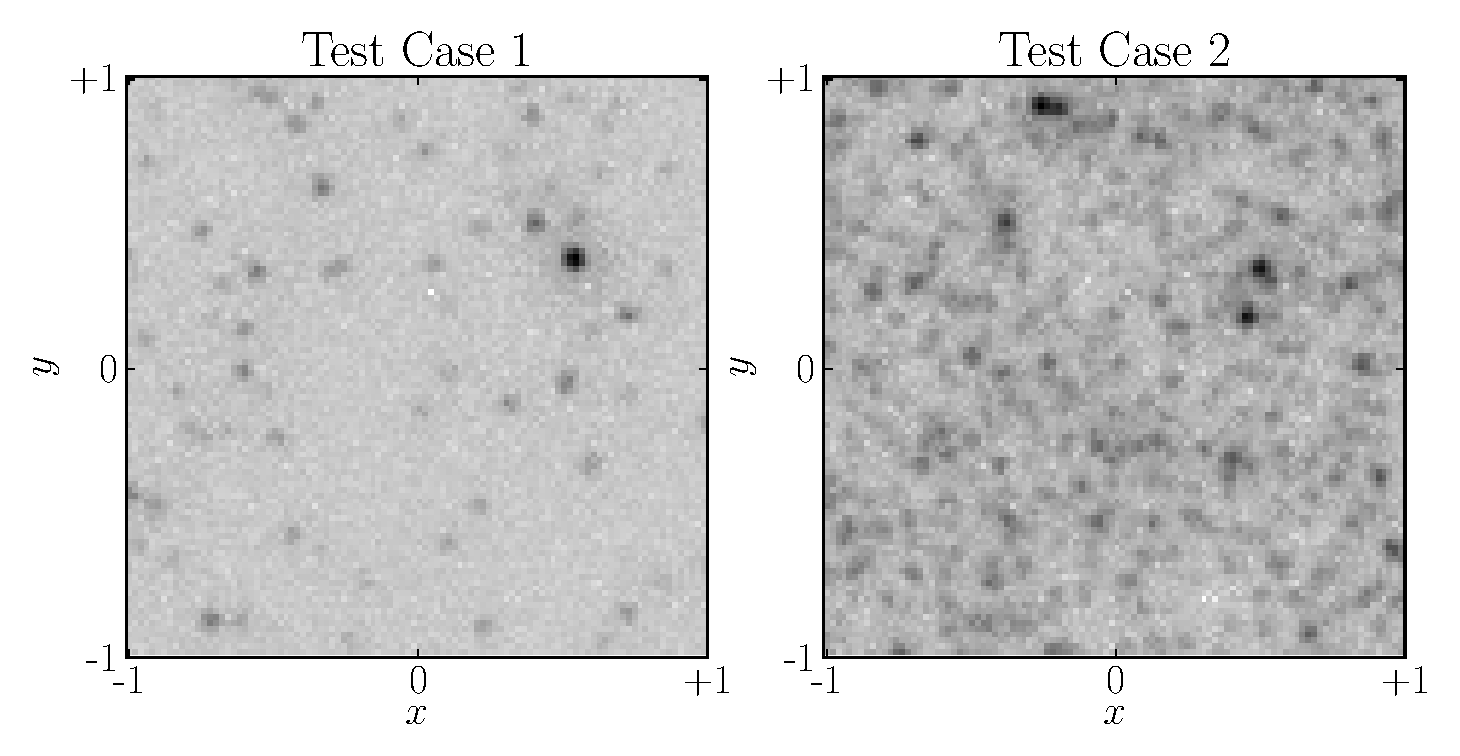
\includegraphics[scale=0.7]{Figures/test_cases.eps}
\caption{Two simulated images.
{\bf Left}: A field containing $\sim$100 stars.
{\bf Right}: A field containing $\sim$1000 stars.\label{fig:simulated_data}}
\end{center}
\end{figure}

\subsection{Test Case 1}

\begin{figure}
\begin{center}
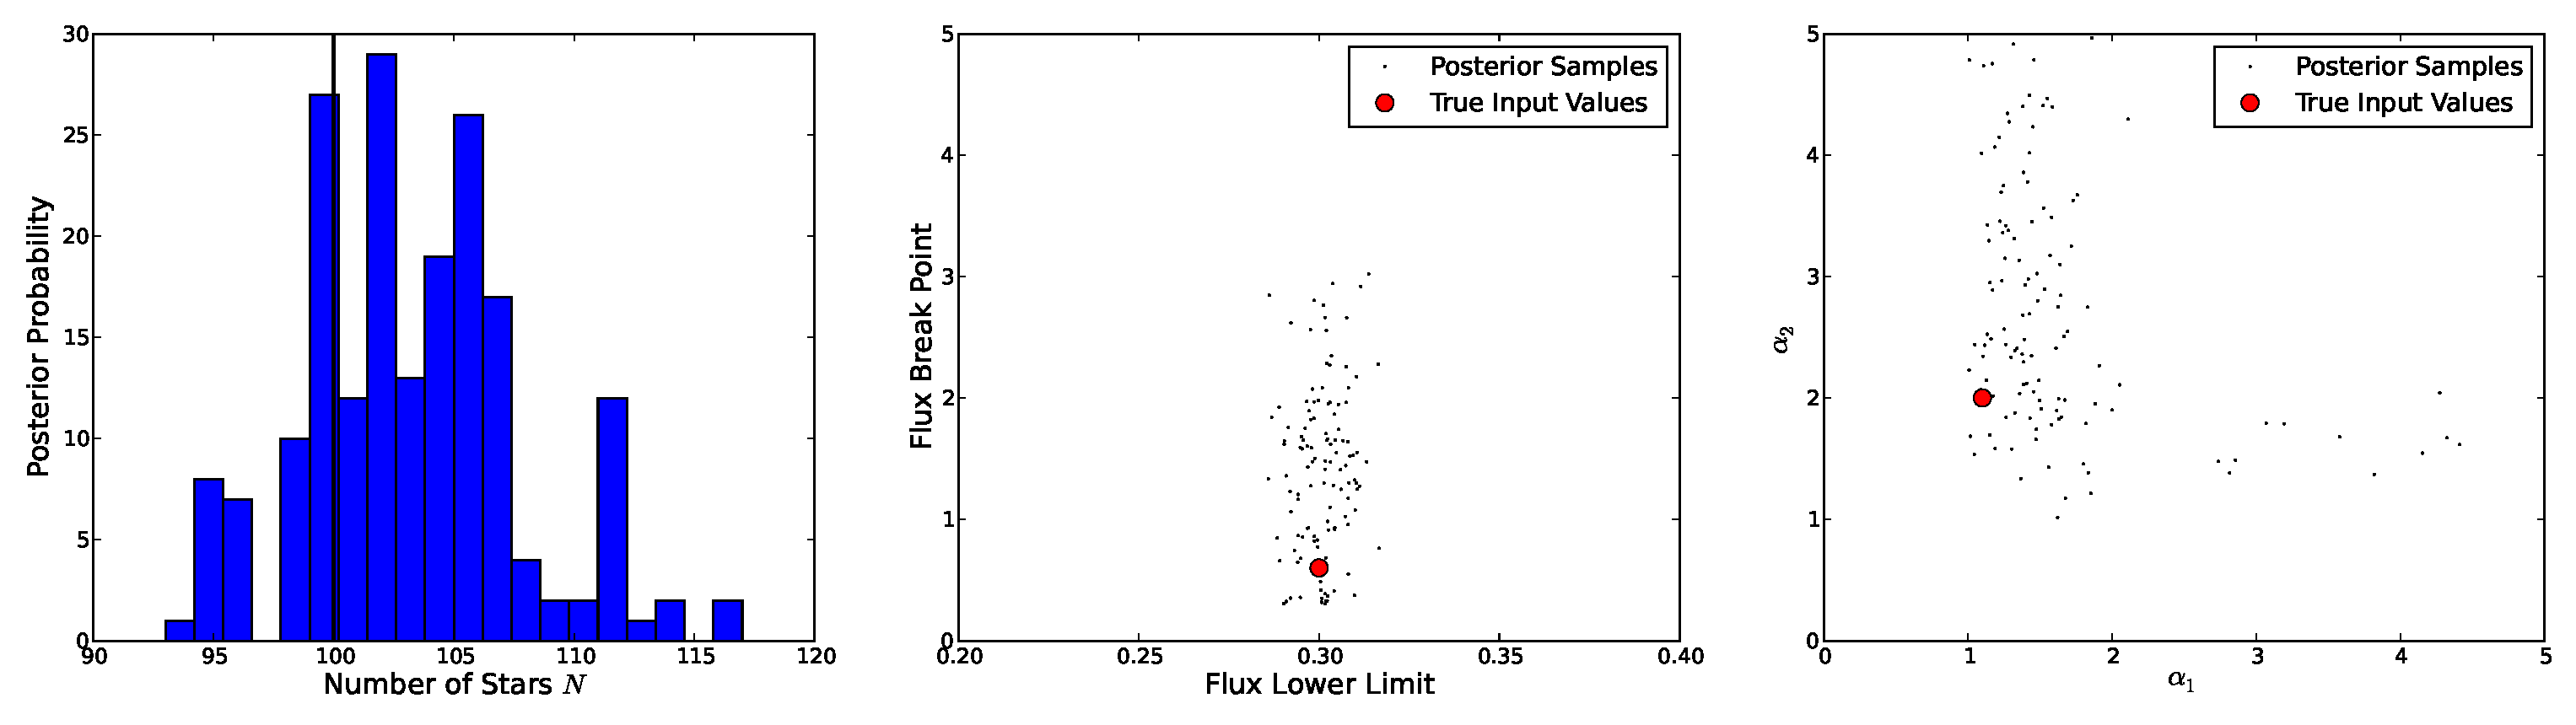
\includegraphics[scale=0.33]{Figures/inference1.eps}
\end{center}
\caption{Inference about the parameters for test case 1.\label{fig:results1}}
\end{figure}

{\bf Show phase transition}\\
{\bf Comment on computational speed}\\
{\bf Show a few catalogs}\\
{\bf Show posterior expected true scene}\\

\subsection{Test Case 2}

\begin{figure}
\begin{center}
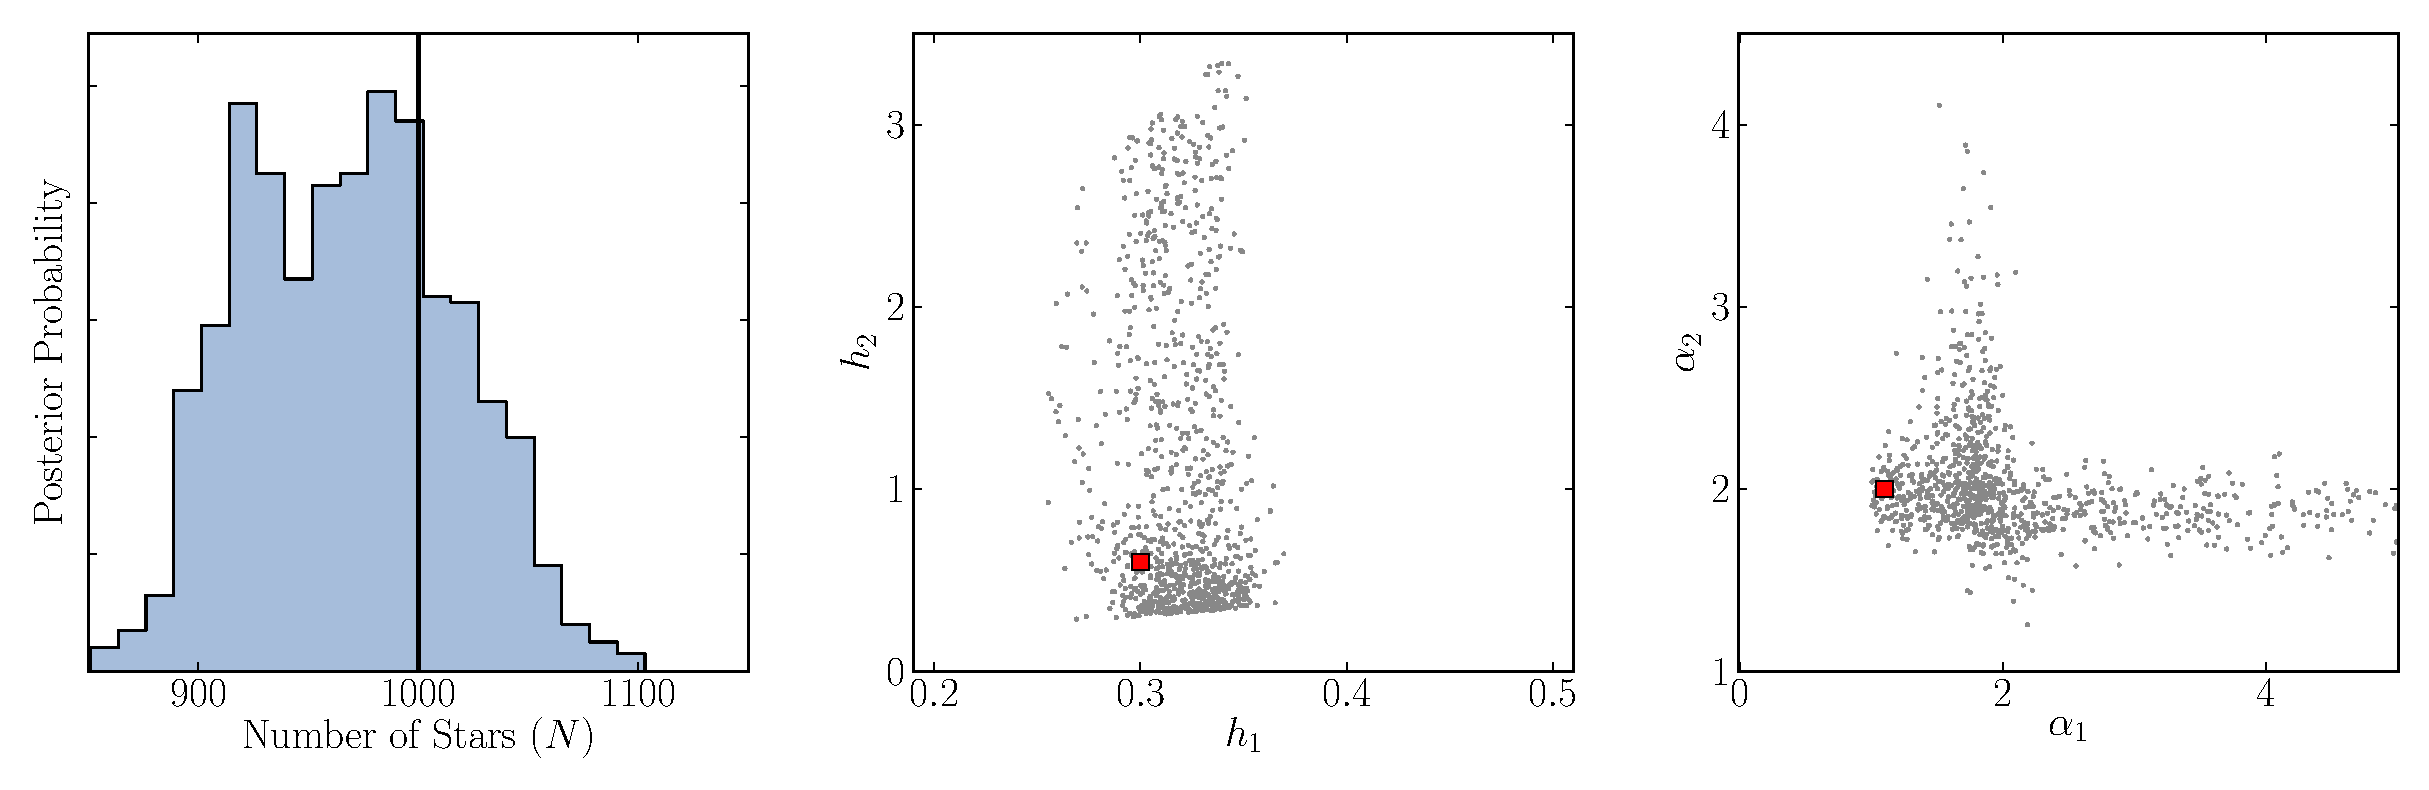
\includegraphics[scale=0.33]{Figures/inference2.eps}
\end{center}
\caption{Inference about the parameters for test case 2.\label{fig:results2}}
\end{figure}



{\bf Show phase transition}\\
{\bf Comment on computational speed}\\
{\bf Show a few catalogs}\\
{\bf Show posterior expected true scene}\\

\begin{figure}
\begin{center}
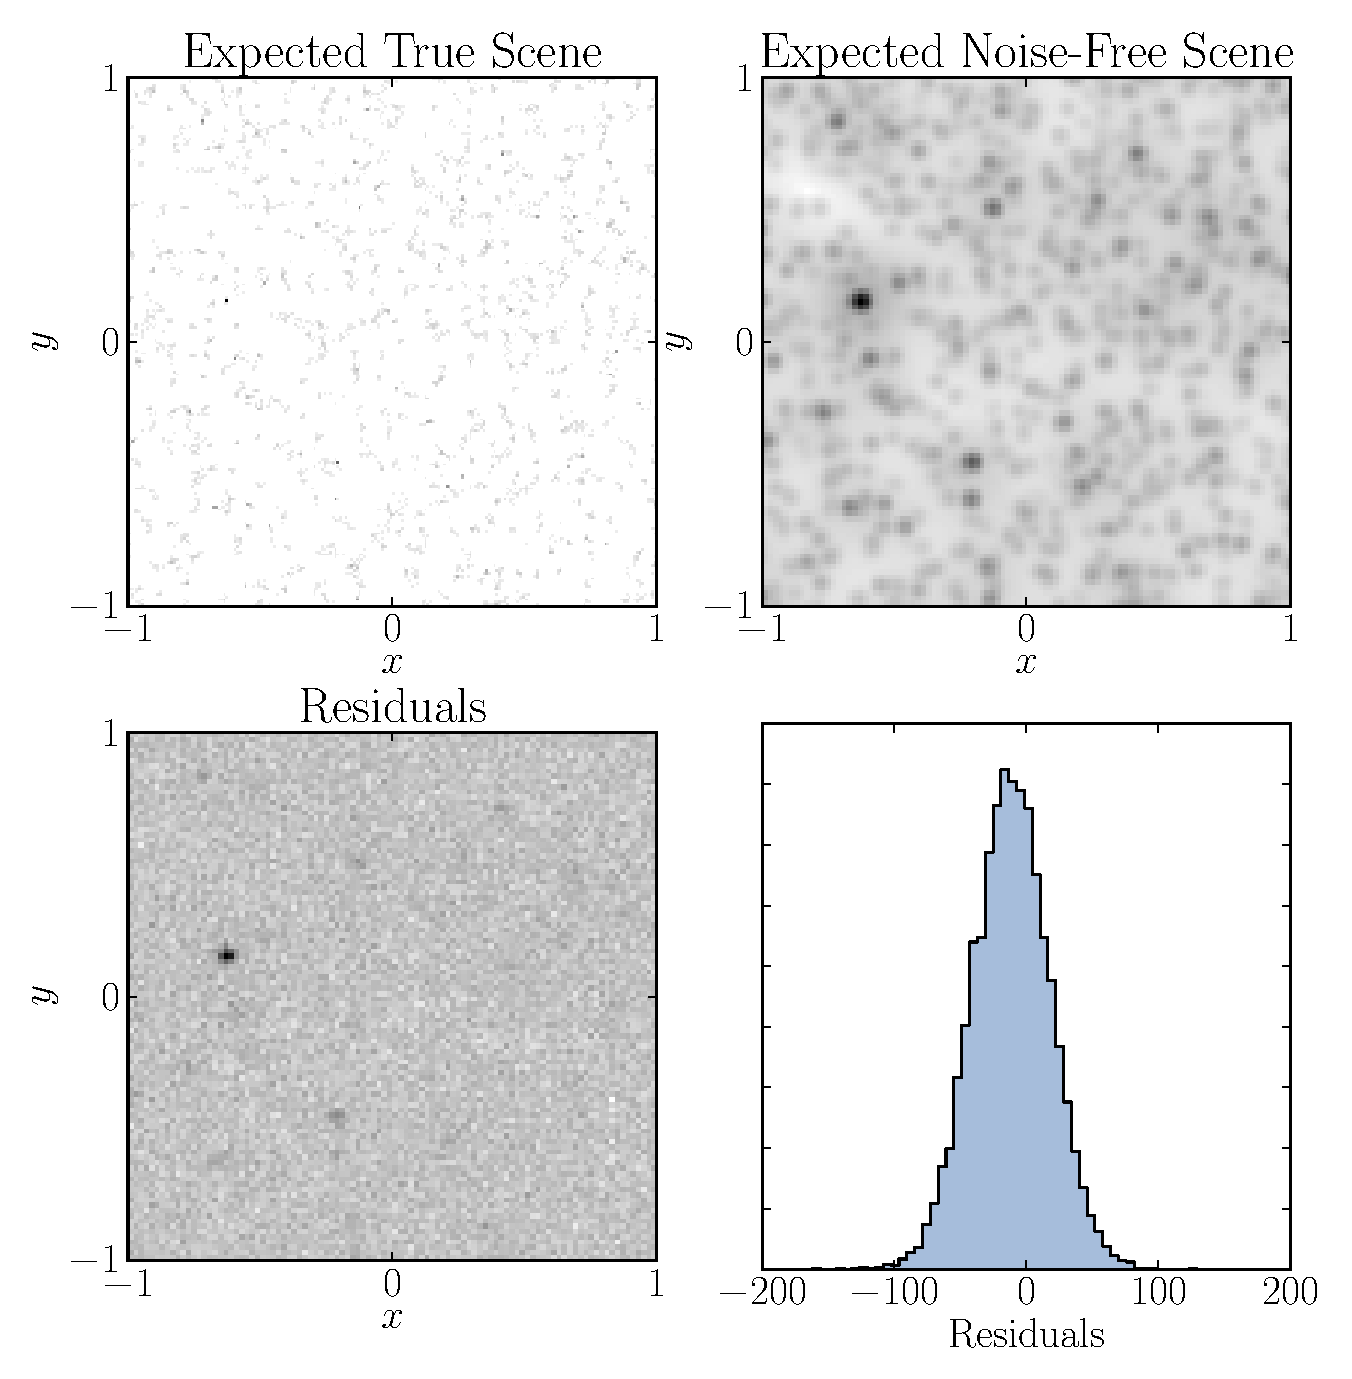
\includegraphics[scale=0.4]{Figures/summaries.eps}
\end{center}
\caption{Summary images for test case 2.\label{fig:summaries}}
\end{figure}

\section{Comparison to SExtractor}

\begin{figure}
\begin{center}
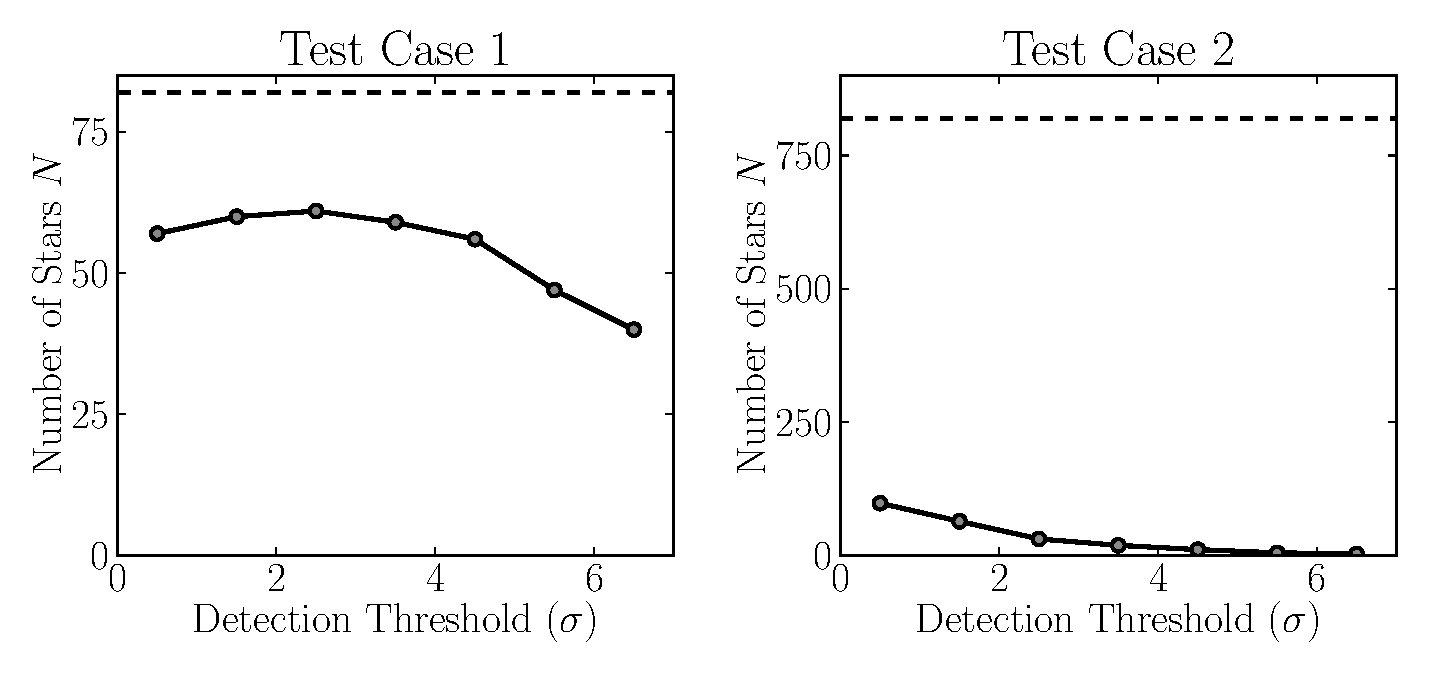
\includegraphics[scale=0.45]{Figures/sex_N.eps}
\end{center}
\caption{The number of stars in the catalogs produced by SExtractor.\label{fig:sex_N}}
\end{figure}


\section{Conclusions}
We can do it. This is important because...

\section{Acknowledgements}
Marshall, Lang, Geraint, Wayne Stewart...


\appendix

\section{Broken Power-Law Distribution}\label{power_law}
The broken power-law distribution is based on a straightforward extension
to a simple power-law distribution (also known as a Pareto distribution,
particularly in the statistics literature). The power-law distribution for a
variable $x$ (given a lower cutoff $x=h$ and a slope $\alpha$) is defined by:
\begin{eqnarray}
p(x) &\propto&
\left\{
\begin{array}{lcr}
0, & & x < h \\
x^{-\alpha - 1} & & x \geq h.
\end{array}
\right.
\end{eqnarray}
In contrast, the broken power-law distribution for a variable $x$ is defined by
a lower cutoff $x=h_1$, two slopes $\{\alpha_1, \alpha_2\}$ and a break point
$x=h_2$:
\begin{eqnarray}
p(x) &\propto&
\left\{
\begin{array}{lcrl}
0, & & x < h_1 & \\
x^{-\alpha_1 - 1} & & h_1 \leq x \leq h_2 & \\
x^{-\alpha_2 - 1} & & x > h_2 & .
\end{array}
\right.
\end{eqnarray}
The free parameters of the broken power-law are:
\begin{eqnarray}
\beta = \{h_1, h_2, \alpha_1, \alpha_2\}.
\end{eqnarray}
With normalising terms included, the proportionality becomes an equality:
\begin{eqnarray}
p(x) &=&
\left\{
\begin{array}{lcr}
0, & & x < h_1 \\
Z_1^{-1}x^{-\alpha_1 - 1}, & & h_1 \leq x \leq h_2 \\
Z_2^{-1}x^{-\alpha_2 - 1}, & & x > h_2.
\end{array}
\right.
\end{eqnarray}
Two conditions will be used to determine the normalizers $Z_1$ and $Z_2$.
Firstly, the probability density function (PDF) should be continuous at $x=h_2$:
\begin{eqnarray}
Z_1^{-1}h_2^{-\alpha_1 - 1} &=& Z_2^{-1}h_2^{-\alpha_2 - 1}\\
\implies
Z_2 &=& Z_1h_2^{\alpha_1-\alpha_2}
\end{eqnarray}
The second condition is that the total probability must be 1:
\begin{eqnarray}
\int_{h_1}^{h_2} Z_1^{-1} x^{-\alpha_1 - 1} \, dx
+
\int_{h_2}^\infty Z_2^{-1} x^{-\alpha_2 - 1} \, dx
&=& 1 \\
Z_1^{-1}\alpha_1^{-1}\left[h_1^{-\alpha_1} - h_2^{-\alpha_1}\right]
+
Z_2^{-1}\alpha_2^{-1}h_2^{-\alpha_2}
&=& 1 \\
Z_1^{-1}\alpha_1^{-1}\left[h_1^{-\alpha_1} - h_2^{-\alpha_1}\right]
+
Z_1^{-1}h_2^{\alpha_2-\alpha_1}\alpha_2^{-1}h_2^{-\alpha_2}
&=& 1
\end{eqnarray}
\begin{eqnarray}
\implies
Z_1 &=& \alpha_1^{-1}\left[h_1^{-\alpha_1} - h_2^{-\alpha_1}\right]
+
h_2^{-\alpha_1}\alpha_2^{-1}.
\end{eqnarray}
The cumulative distribution (CDF) is a useful property of a probability
distribution and is given by the antiderivative of the PDF:
\begin{eqnarray}
P(X \leq x) = F(x) &=& 
\left\{
\begin{array}{lcr}
0, & & x < h_1 \\
(Z_1\alpha_1)^{-1}\left(h_1^{-\alpha_1} - x^{-\alpha_1}\right), & & h_1 \leq x \leq h_2 \\
1 - (Z_2\alpha_2)^{-1}x^{-\alpha_2}, & & x > h_2 
\end{array}
\right.
.
\end{eqnarray}
The inverse of the CDF is also useful and is given by:
\begin{eqnarray}
F^{-1}(u) &=& 
\left\{
\begin{array}{lcr}
\left[h_1^{-\alpha_1} - uZ_1\alpha_1\right]^{-1/\alpha_1}, & & 0 < u < 1 - (Z_2\alpha_2)^{-1}h_2^{-\alpha_2}\\
\left[Z_2\alpha_2(1-u)\right]^{-1/\alpha_2},& & 1 - (Z_2\alpha_2)^{-1}h_2^{-\alpha_2}< u < 1
\end{array}
\right.
.
\end{eqnarray}
An example of a broken power-law distribution is shown in Figure~\ref{fig:powerlaw}.
\begin{figure}[h!]
\begin{center}
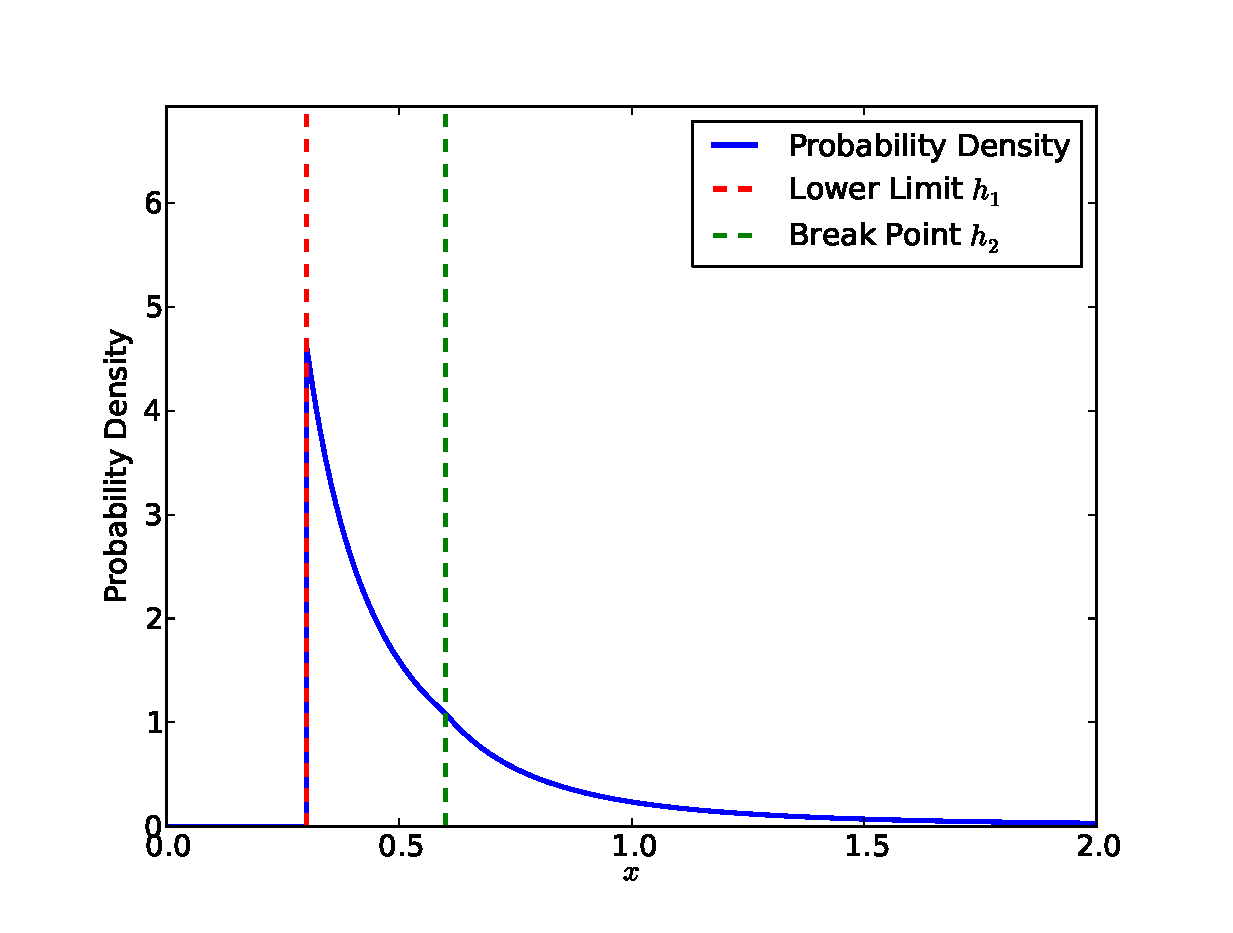
\includegraphics[scale=0.5]{Figures/broken.eps}
\caption{A broken power-law distribution. The parameter values for this
particular PDF were
$\{h_1, h_2, \alpha_1, \alpha_2\} = \{0.3, 0.6, 1.1, 2\}$, i.e. the same
parameter values used to make the simulated data.
\label{fig:powerlaw}}
\end{center}
\end{figure}


\section{Pixel Convolved PSF}
{\bf Do people need to be schooled on this? I did...}
Consider a ``true image'' $f_0(x, y)$ with infinite resolution. We now model how
this image gives rise to the observed data. First, it is convolved with a
PSF $g(\delta_x, \delta_y)$ (assumed normalized to 1) to give the blurred image:
\begin{eqnarray}
f_{\rm{blurred}}(x, y) &=& \iint f_0(x-\delta_x, y-\delta_y)
g(\delta_x, \delta_y) \, d\delta_x \, d\delta_y \label{blur}
\end{eqnarray}
Then, we observe the blurred image with a certain pixellation. Consider a pixel.
The true flux $F$ within the pixel is:
\begin{eqnarray}
F &=& \iint_{\rm pixel} f_{\rm blurred}(x, y) \,dx'\,dy'\\
&=& \iint f_{\rm blurred}(x, y)\mathbbm{1}\left[(x,y) \in \textnormal{pixel}
\right] \,dx\,dy \label{pixel}
\end{eqnarray}
Now consider $F$ as a function of the central location $(x_c, y_c)$ of the
pixel.

\section{Usage}
Software can be obtained from {\tt http://github.com/dfm/star-field/}

\section{Proposal Distributions}

\begin{table}
\begin{center}
\begin{tabular}{|c|c|c|}
\hline
Parameter & Proposal & Notes\\
\hline
$N$ & $N \to N + \delta_N$ & Generate $\delta_N$ new stars from prior given
$\beta$\\
$N$ & $N \to N - \delta_N$ & Remove $\delta_N$ stars at random\\
$\beta$ & $\beta \to \beta + \delta_\beta$ & Move stars' fluxes along with
$\beta$\\
$\beta$ & $\beta \to \beta + \delta_\beta$ & Stars' fluxes fixed, put extra
term in acceptance probability \\
$(x_i,y_i)$ & $(x_i,y_i) \to (x_i,y_i)+(\delta_x, \delta_y)$ & Can move $>1$ star
in a single step \\
$f$ & $f \to f + \delta_f$ & Can move $>1$ stars' fluxes in a single step\\
\hline
\end{tabular}
\end{center}
\caption{All $\delta$ parameters are drawn from multi-scale distibutions such
that the largest steps are of order the prior width, and the smallest steps
are of order $10^{-6}$ times the prior width.\label{proposals}}
\end{table}

See Table~\ref{proposals} for a list of current proposal distributions.




%\subsection{Future Possibilities}
%{\bf Hogg}: {\it I think this problem is important enough and general enough
%that we should spend some time working on some ideas there.  If we can sample
%over image explanations, our powers in astronomy will be awesome
%beyond our wildest imaginings.}

%\subsection{Genetic Moves}
%Here I will sketch some ideas...




\begin{thebibliography}{99}
\bibitem[Bertin and 
Arnouts(1996)]{sextractor} Bertin, E., Arnouts, S.\ 1996.\ SExtractor: Software for source extraction.\ Astronomy and Astrophysics Supplement Series 117, 393-404.

\bibitem[\protect\citeauthoryear{Brewer, P{\'a}rtay, 
\& Cs{\'a}nyi}{2011}]{dnest} Brewer B.~J., P{\'a}rtay L.~B.,
Cs{\'a}nyi G., 2011, Statistics and Computing, 21, 4, 649-656. arXiv:0912.2380

\bibitem[Brewer et al.(2011)]{2011MNRAS.412.2521B} Brewer, B.~J., Lewis, 
G.~F., Belokurov, V., Irwin, M.~J., Bridges, T.~J., Evans, N.~W.\ 2011.\ 
Modelling of the complex CASSOWARY/SLUGS gravitational lenses.\ Monthly 
Notices of the Royal Astronomical Society 412, 2521-2529

\bibitem[Caticha(2009)]{caticha} Caticha, A.\ 2009.\ 
Quantifying Rational Belief.\ American Institute of Physics Conference 
Series 1193, 60-68. 

\bibitem[Cox(1946)]{cox} Cox, R.~T., 1946, Probability, Frequency, and Reasonable Expectation. 1946. American Journal of Physics 14 14, 1-13.

\bibitem[Feroz et al.(2011)]{2011MNRAS.415.3462F} Feroz, F., Balan, S.~T., 
Hobson, M.~P.\ 2011.\ Detecting extrasolar planets from stellar radial 
velocities using Bayesian evidence.\ Monthly Notices of the Royal 
Astronomical Society 415, 3462-3472. 

\bibitem[\protect\citeauthoryear{Feroz, Hobson, 
\& Bridges}{2009}]{multinest} Feroz F., Hobson M.~P., Bridges M., 2009, MNRAS, 398, 1601 

\bibitem[\protect\citeauthoryear{Green}{1995}]{rjmcmc}
Green, P.~J., 1995, Reversible Jump Markov Chain Monte Carlo Computation and Bayesian Model Determination, Biometrika 82 (4): 711–732.

\bibitem[Hogg(2012)]{hogg} Hogg, D.~W.\ 2012.\ Data analysis 
recipes: Probability calculus for inference.\ ArXiv e-prints 
arXiv:1205.4446. 

\bibitem[Hogg and Lang(2011)]{2011EAS....45..351H} Hogg, D.~W., Lang, D.\ 
2011.\ Telescopes don't make catalogues!.\ EAS Publications Series 45, 
351-358. 

\bibitem[Irwin(1985)]{irwin} Irwin, M.~J.\ 1985, \mnras, 214, 
575 

\bibitem[Jaynes(2003)]{jaynes} Jaynes, E.~T., 2003, Probability Theory: The
Logic of Science, ISBN 0521592712, Cambridge University Press, June 2003.

\bibitem[Kelly et al.(2008)]{2008ApJ...682..874K} Kelly, B.~C., Fan, X., 
\& Vestergaard, M.\ 2008, ApJ, 682, 874 

\bibitem[Mackay(2003)]{mackay} Mackay, D.~J.~C., 2003, Information Theory,
Inference and Learning Algorithms, Cambridge University Press, UK.

\bibitem[\protect\citeauthoryear{Skilling}{1998}]{massinf} 
Skilling J., 1998, Massive Inference and Maximum Entropy, in Maximum Entropy 
and Bayesian Methods, Kluwer Academic Publishers, Dordrecht/Boston/London p.14
\end{thebibliography}

\end{document}

